\begin{figure*}[t]
\centering
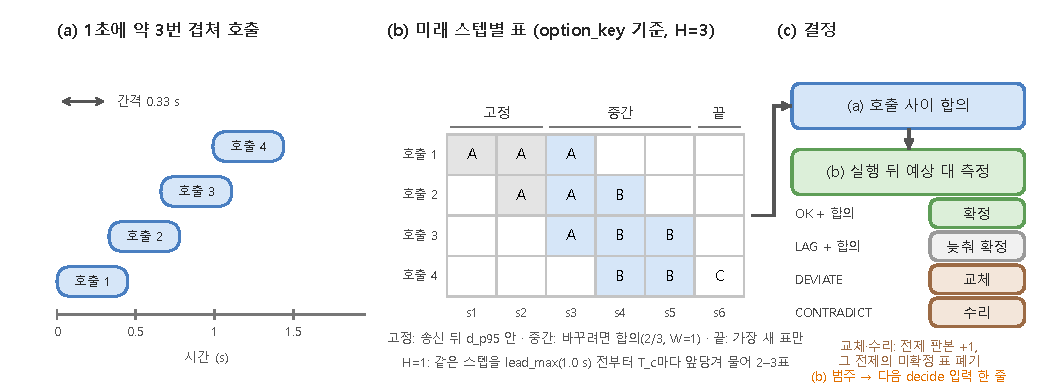
\includegraphics[width=\linewidth]{figures/m4_commit.pdf}
\caption{\textbf{M4 확정 규칙.} (a) Jev를 약 0.33\,s 간격으로 겹쳐 부른다(지연은 E0에서 실측). (b) 답을 미래 스텝별 표로 모으고, RTC의 구간을 이산판으로 옮겨 고정(Jev p95 지연 길이), 중간(바꾸려면 합의 필요), 끝(최신 표 가확정)으로 나눈다. 표의 보기는 \texttt{option\_key}로 센다. (c) 호출 사이 합의(a)와 실행 뒤 코드 예상 상태 대 측정 상태 비교(b)가 모두 맞으면 확정하고, (b)가 어긋나면 전제 판본을 올려 그 전제에 기댄 표를 무효화한 뒤 교체·수리를 고른다. 표의 A--D는 설명용 예시다.}
\label{fig:m4}
\end{figure*}
